\section{The Tank}
\label{sec:tank}
The main component of the SK detector is a cylindrical stainless steel tank, with a diameter of 39 m and a height of 42 m, which is filled with about 50 ktons of water.  The structure of the detector is shown in \cref{fig:sk_detector_diagrams}.  The tank is segmented into an inner detector (ID), with a diameter 33.8 m and a height of 36.2 m, which hold 32 ktons of water, and an outer detector (OD) which is the region of the tank outside the ID.  The ID is the primary detector used for most physics analyses, while the OD is primarily used as an active cosmic ray veto.  The ID and OD are separated from one another by a cylindrical PMT support structure.  On the inner surface of the support structure, 11,146 inward-facing 20 inch PMTs, giving a coverage of about 40\% are mounted to observe activity in the ID (for SK-II half as many PMTs were used in the ID).  The outer surface of the support structure is instrumented with 1885 outward-facing 8 inch PMTs to observe the OD.  Lightproof Tyvek sheeting on both surfaces of the PMT structure optically separates the ID from the OD.  It also results in a 55 cm this dead space between the ID and the OD, from which light cannot escape.  The Tyvek sheeting is black on the side facing into the ID, in order to reduce reflections which would diminish reconstruction accuracy.  On the side facing the OD, conversely, the Tyvek sheeting is white, in order to increase reflections.  This is done to improve light collection efficiency in the OD, the compensate for its lower PMT coverage.  Scattered light in the OD is also much less problematic for physics goals compared to scattered light in the ID. \par
The PMTs are very sensitive to magnetic fields, and the about 450 mG geomagnetic field at the SK detector site would significantly reduce their efficiency.  Therefore, 26 sets of horizontal and verticle Helmholtz coils are arranged around the inner surface of the tank.  These reduce the magnetic field in the tank to about 50 mG, which results in an estimated about 1-2\% effect on the collection efficiency of the ID PMTs. 

\begin{figure*}
\centering
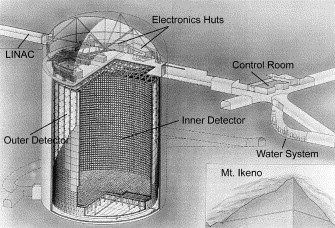
\includegraphics[width=0.8\textwidth]{figures/sk_detector_under_mountain.jpg}
\caption{Structure of the SK detector. \cite{Fukuda:2002uc}}
\label{fig:sk_detector_diagrams} 
\end{figure*}

\begin{figure*}
\centering
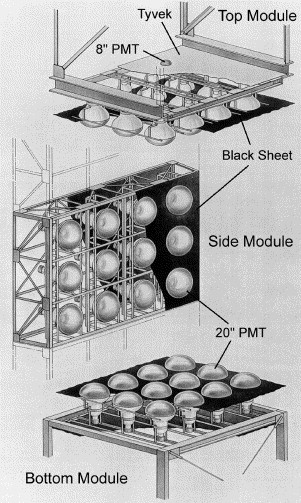
\includegraphics[width=0.8\textwidth]{figures/pmt_support_structure.jpg}
\caption{PMT support structure. \cite{Fukuda:2002uc}}
\label{fig:pmt_support_structure} 
\end{figure*}